\documentclass[8pt]{article}
\usepackage{amssymb}
\usepackage{hyperref}
\usepackage{pgfplots}
\usepackage{placeins}
\usepackage{array}
\usepackage{tikz}
\usepackage{circuitikz}
\usetikzlibrary{circuits.logic.US, circuits.ee.IEC, positioning}
\usepackage{amsmath}
\usepackage{graphicx}
\usepackage[T1]{fontenc}
\usepackage[utf8]{inputenc}
\usepackage{listings}
\usepackage{xcolor}
\usepackage{geometry}
\input{kvmacros.tex}
\geometry{margin=0.4in}

\lstdefinelanguage{SystemVerilog}{
  morekeywords={module, endmodule, logic, bit, int, enum, struct,
    always_ff, always_comb, initial, final, interface, modport, property,
    assert, class, rand, constraint, generate, endgenerate, if, else, begin, end},
  sensitive=true,
  morecomment=[l]{//},
  morecomment=[s]{/*}{*/},
  morestring=[b]",
}

\lstset{
  language=SystemVerilog,
  basicstyle=\ttfamily\footnotesize,
  keywordstyle=\color{blue}\bfseries,
  commentstyle=\color{gray}\itshape,
  stringstyle=\color{red},
  frame=single,
  breaklines=true,
  postbreak=\mbox{\textcolor{red}{$\hookrightarrow$}\space},
}

% demuxes and muxes
% - explanation of functionality
% encoders and decoders
% - explanation of functionality
% static 1 and staic 0 hazards
% k-maps
% - detecting static hazards
% - representing as PoS and SoP
% On and off sets
% SystemVerilog: structural vs dataflow vs behavioral

\begin{document}
\noindent \makebox[1.5in]{\hrulefill} \\[10pt]
\section*{Multiplexer}

Multiplexers select one of $2^n$ input lines based on
the binary representation of the $n$ selection lines. For example,
this 3-8 multiplexer selects the input $x_i$ corresponding
to the binary number $y_2y_1y_0$.
\begin{center}
    \tikzstyle{branch}=[fill,shape=circle,minimum size=3pt,inner sep=0pt]
    \begin{tikzpicture}[scale=0.5, transform shape]

        % nodes
        \node (y1) at (1,0) {$y_0$};
        \node (y2) at (2,0) {$y_1$};
        \node (y3) at (3,0) {$y_2$};
        \node[not gate US, draw, rotate=-90] at ($(y1)+(0.5,-1)$) (noty1) {};
        \node[not gate US, draw, rotate=-90] at ($(y2)+(0.5,-1)$) (noty2) {};
        \node[not gate US, draw, rotate=-90] at ($(y3)+(0.5,-1)$) (noty3) {};

        \node (x1) at (0,-2) {$x_0$};
        \node (x2) at (0,-3) {$x_1$};
        \node (x3) at (0,-4) {$x_2$};
        \node (x4) at (0,-5) {$x_3$};
        \node (x5) at (0,-6) {$x_4$};
        \node (x6) at (0,-7) {$x_5$};
        \node (x7) at (0,-8) {$x_6$};
        \node (x8) at (0,-9) {$x_7$};

        \node[and gate US, draw, logic gate inputs=nnnn] at ($(y3)+(5,-2.25)$) (And1) {};
        \node[and gate US, draw, logic gate inputs=nnnn] at ($(And1)+(0,-1)$) (And2) {};
        \node[and gate US, draw, logic gate inputs=nnnn] at ($(And2)+(0,-1)$) (And3) {};
        \node[and gate US, draw, logic gate inputs=nnnn] at ($(And3)+(0,-1)$) (And4) {};
        \node[and gate US, draw, logic gate inputs=nnnn] at ($(And4)+(0,-1)$) (And5) {};
        \node[and gate US, draw, logic gate inputs=nnnn] at ($(And5)+(0,-1)$) (And6) {};
        \node[and gate US, draw, logic gate inputs=nnnn] at ($(And6)+(0,-1)$) (And7) {};
        \node[and gate US, draw, logic gate inputs=nnnn] at ($(And7)+(0,-1)$) (And8) {};
        \node[or gate US, draw, logic gate inputs=nnnnnnnn, anchor=input 1] at ($(And1.output -| And2.output)+(2,-2.75)$) (Or1) {};

        % draw nodes to NOT
        \foreach \i in {1,2,3} {
                \path (y\i) -- coordinate (punt\i) (y\i |- noty\i.input);
                \draw (punt\i) node[branch] {} -| (noty\i.input);
            }

        % connect x_i to AND_i
        \foreach \i in {1,2,3,4,5,6,7,8} {
                \draw (x\i) -- (And\i.input 1);
            }

        % y1
        \draw (y1 |- And5.input 2) node[branch] {} -- (And5.input 2);
        \draw (y1 |- And6.input 2) node[branch] {} -- (And6.input 2);
        \draw (y1 |- And7.input 2) node[branch] {} -- (And7.input 2);
        \draw (y1) |- (And8.input 2);
        \draw (noty1 |- And1.input 2) node[branch] {} -- (And1.input 2);
        \draw (noty1 |- And2.input 2) node[branch] {} -- (And2.input 2);
        \draw (noty1 |- And3.input 2) node[branch] {} -- (And3.input 2);
        \draw (noty1) |- (And4.input 2);

        % y2
        \draw (y2 |- And3.input 3) node[branch] {} -- (And3.input 3);
        \draw (y2 |- And4.input 3) node[branch] {} -- (And4.input 3);
        \draw (y2 |- And7.input 3) node[branch] {} -- (And7.input 3);
        \draw (y2) |- (And8.input 3);
        \draw (noty2 |- And1.input 3) node[branch] {} -- (And1.input 3);
        \draw (noty2 |- And2.input 3) node[branch] {} -- (And2.input 3);
        \draw (noty2 |- And5.input 3) node[branch] {} -- (And5.input 3);
        \draw (noty2) |- (And6.input 3);

        % y3
        \draw (y3 |- And2.input 4) node[branch] {} -- (And2.input 4);
        \draw (y3 |- And4.input 4) node[branch] {} -- (And4.input 4);
        \draw (y3 |- And6.input 4) node[branch] {} -- (And6.input 4);
        \draw (y3) |- (And8.input 4);
        \draw (noty3 |- And1.input 4) node[branch] {} -- (And1.input 4);
        \draw (noty3 |- And3.input 4) node[branch] {} -- (And3.input 4);
        \draw (noty3 |- And5.input 4) node[branch] {} -- (And5.input 4);
        \draw (noty3) |- (And7.input 4);

        % AND
        \draw (And1.output) -- ([xshift=0.8cm]And1.output) |- (Or1.input 1);
        \draw (And2.output) -- ([xshift=0.6cm]And2.output) |- (Or1.input 2);
        \draw (And3.output) -- ([xshift=0.4cm]And3.output) |- (Or1.input 3);
        \draw (And4.output) -- ([xshift=0.2cm]And4.output) |- (Or1.input 4);
        \draw (And5.output) -- ([xshift=0.2cm]And5.output) |- (Or1.input 5);
        \draw (And6.output) -- ([xshift=0.4cm]And6.output) |- (Or1.input 6);
        \draw (And7.output) -- ([xshift=0.6cm]And7.output) |- (Or1.input 7);
        \draw (And8.output) -- ([xshift=0.8cm]And8.output) |- (Or1.input 8);

        % OR
        \draw (Or1.output) -- ([xshift=0.5cm]Or1.output) node[above] {$z$};

    \end{tikzpicture}
\end{center}
Demultiplexers perform the inverse, accepting $2^n$ input lines and
selecting one for output based on the binary representation of the
$n$ selection lines.

\section*{Decoder}

Decoders convert an input binary signal to an output signal.
\begin{center}
    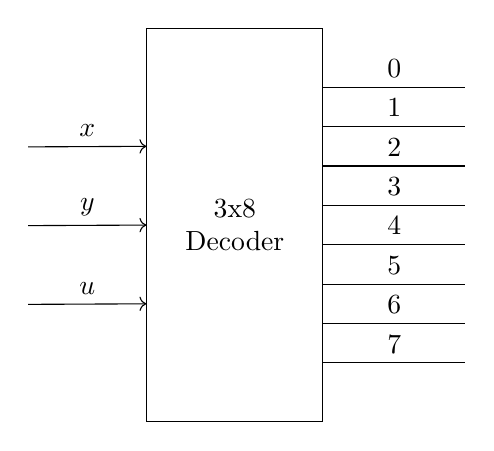
\begin{tikzpicture}
        %coordinates
        \coordinate (orig)   at (0,0);

        \coordinate (Dec) at (1,4);

        \coordinate (x) at ($(Dec) + (-1.5,3.5)$);
        \coordinate (y) at ($(x) + (0,-1)$);
        \coordinate (u) at ($(y) + (0,-1)$);

        %nodes
        \node[draw, minimum width=2cm, minimum height=5cm, anchor=south west, text width=2cm, align=center] (A) at (Dec) {3x8\\Decoder};
        % \node[or gate US, draw, logic gate inputs=nnnn] at ($(A)+(4.5,1)$) (B) {};
        % \node[or gate US, draw, logic gate inputs=nnnn] at ($(A)+(4.5,-1)$) (C) {};

        %edges
        \draw[->] (x) -- node[above]{$x$} ($(A.180) + (0,1)$);
        \draw[->] (y) -- node[above]{$y$} ($(A.180) + (0,0)$);
        \draw[->] (u) -- node[above]{$u$} ($(A.180) + (0,-1)$);

        \draw ($(A.0) + (0, 1.75)$) -- node[above]{0} ($(A.0) + (1.8, 1.75)$);
        \draw ($(A.0) + (0, 1.25)$) -- node[above]{1} ($(A.0) + (1.8, 1.25)$); % |- (B.input 1);
        \draw ($(A.0) + (0, 0.75)$) -- node[above]{2} ($(A.0) + (1.8, 0.75)$); % |- (B.input 2);
        \draw ($(A.0) + (0, 0.25)$) -- node[above]{3} ($(A.0) + (1.8, 0.25)$); % |- (C.input 1);
        \draw ($(A.0) + (0, -0.25)$) -- node[above]{4} ($(A.0) + (1.8, -0.25)$); % |- (B.input 3);
        \draw ($(A.0) + (0, -0.75)$) -- node[above]{5} ($(A.0) + (1.8, -0.75)$); % |- (C.input 2);
        \draw ($(A.0) + (0, -1.25)$) -- node[above]{6} ($(A.0) + (1.8, -1.25)$); % |- (C.input 3);
        \draw ($(A.0) + (0, -1.75)$) -- node[above]{} ($(A.0) + (1.8, -1.75)$); % |- (C.input 4);
        \draw ($(A.0) + (0, -1.75)$) -- node[above]{7} ($(A.0) + (1.8, -1.75)$); % |- (B.input 4);

        % \draw (C.output) -- node[above]{$U$} ($(C.output) + (1, 0)$);
        % \draw (B.output) -- node[above]{$R$} ($(B.output) + (1, 0)$);

        %\draw[->] (A.270) -- node[above]{} (B.90);
        %\draw[->] (C.270) -- node[above]{} (D.90);

        %\draw[->] (A) -| node[above]{} ($(E.180) + (-2,0.3)$) -- node[above]{} ($(E.180) + (0,0.3)$);
        %\draw[->] (B) -| node[above]{} ($(F.180) + (-2,0.3)$) -- node[above]{} ($(F.180) + (0,0.3)$);
        %\draw[->] (C) -| node[above]{} ($(E.180) + (-3,-0.3)$) -- node[above]{} ($(E.180) + (0,-0.3)$);
        %\draw[->] (D) -| node[above]{} ($(F.180) + (-2,-0.3)$) -- node[above]{} ($(F.180) + (0,-0.3)$);

        %\draw[->] (B.270) |- node[above]{} ($(F.180) + (-2.5,+ If I email 0.3)$) |- node[above]{} ($(G.180) + (0,0.3)$);
        %\draw[->] (D.270) |- node[above]{} ($(D.270) + (3.3,-0.5)$) |- node[above]{} ($(G.180) + (0,-0.3)$);

        %\draw[->] (E.270) -- node[above]{} (F.90);
        %\draw[->] (F.270) -- node[above]{} (G.90);

        %\draw[->] (E) -- node[above]{$R_0$} ($(E) + (3, 0)$);
        %\draw[->] (F) -- node[above]{$R_1$} ($(F) + (3, 0)$);
        %\draw[->] (G) -- node[above]{$R_2$} ($(G) + (3, 0)$);
        %\draw[->] (G) |- node[above]{} ($(G) + (0, -2)$) -- node[above]{} ($(G) + (1, -2)$) -- node[above]{$R_3$} ($(G) + (3, -2)$);
    \end{tikzpicture}
\end{center}
Encoders perform the inverse, converting the index of the input signal
to a binary number. Since encoders may exhibit unwanted behavior if more than
one input signals are asserted at a time, \emph{priority} encoders will output
the binary representation of the highest-priority input signal for some
notion of priority.

\section*{Static Hazards}
Static hazards occur in combinational logic circuits when a single input change causes a
momentary fluctuation in the output, even though the final output should remain constant.
There are two types of static hazards:
\begin{itemize}
    \item[Static-1] Occurs when the output is supposed to remain at
          logic 1 but momentarily drops to 0.
    \item[Static-0] Occurs when the output is supposed to remain at
          logic 0 but momentarily rises to 1.
\end{itemize}
For example, consider the following circuit diagram for $\neg X \oplus X$:
\begin{center}
    \begin{circuitikz}
        % Inverter
        \node[scale=0.5, not port, anchor=out] (not) at (-1.65, 0.28) {};
        % XOR gate
        \node[xor port] (xor) at (0,0) {};
        % Input labels
        \draw (xor.in 1) -- (not.out);
        \node[left] at (not.in) {$X$};
        \draw (xor.in 2) -- ++(-1,0) node[left] {$X$};
        % Output label
        \draw (xor.out) -- ++(1,0) node[right] {$\neg X \oplus X$};
    \end{circuitikz}
\end{center}
In this circuit, $X$ is the input and $\neg X$ is the negated
input, and $\neg X \oplus X$ is the output of the XOR gate. The output
will always be 1, except for when the propogation delay from the NOT gate cause a
momentary fluctuation.


\section*{Karnaugh Map}
To find the PoS and SoP representations:
\begin{itemize}
    \item[SoP] Group the 1s in the K-map into the largest
          possible groups of 1, 2, 4, 8, etc. Each group represents
          a product term.
    \item[PoS] Group the 0s in the K-map into the largest
          possible groups of 1, 2, 4, 8, etc. Each group represents
          a sum term.
\end{itemize}
To detect static hazards from the K-map, look for adjacent
cells with the same value but covered by different groups.
\begin{center}
    \karnaughmap{4}{$f(A,B,C,D):$}{{$A$}{$C$}{$B$}{$D$}}{1100110001001100}
    {
        \put(2,3.5){\color{red}\oval(3.9,0.9)}
        \put(2,4){\color{blue}\oval(1.9,1.9)[b]}
        \put(2,0){\color{blue}\oval(1.9,1.9)[t]}
        \put(3,4){\color{orange}\oval(1.9,1.9)[b]}
        \put(3,0){\color{orange}\oval(1.9,1.9)[t]}
    }
\end{center}
\begin{align}
    {\color{red}\neg A \neg B} + {\color{blue}\neg B D} + {\color{orange}\neg B C}
\end{align}

\section*{SystemVerilog Modeling}
Structural modeling describes the circuit in terms of its
components and their interconnections using logic gates. This
is the most concrete form of modeling.
\begin{lstlisting}[language=SystemVerilog, caption=Structural Modeling Example]
module and_gate (output wire Y, input wire A, B);
    and (Y, A, B);
endmodule

module top;
    wire A, B, Y;
    and_gate u1 (.Y(Y), .A(A), .B(B));
endmodule
\end{lstlisting}
Dataflow modeling describes the circuit in terms of the
flow of data using continuous assignments. It uses
operators to define the relationships between inputs
and outputs.
\begin{lstlisting}[language=SystemVerilog, caption=Dataflow Modeling Example]
module and_gate (output wire Y, input wire A, B);
    assign Y = A & B;
endmodule

module top;
    wire A, B, Y;
    and_gate u1 (.Y(Y), .A(A), .B(B));
endmodule
\end{lstlisting}
Behavioral modeling describes the circuit in terms of its
behavior using procedural blocks. It uses constructs like
`always', `if', and `?' to define how the output changes in
response to changes in the input. This is the most
abstract form of modeling.
\begin{lstlisting}[language=SystemVerilog, caption=Behavioral Modeling Example]
module and_gate (output reg Y, input wire A, B);
    always @ (A or B) begin
        Y = A & B;
    end
endmodule

module top;
    wire A, B;
    reg Y;
    and_gate u1 (.Y(Y), .A(A), .B(B));
endmodule
\end{lstlisting}

\end{document}